\documentclass[a4paper,12pt]{article} 
\usepackage[top=15mm,left=12.5mm, right=12.5mm]{geometry}

% Рисунки
\usepackage{graphicx}
\usepackage{wrapfig}

%  Русский язык
\usepackage[T2A]{fontenc}			% кодировка
\usepackage[utf8]{inputenc}			% кодировка исходного текста
\usepackage[english,russian]{babel}	% локализация и переносы

% Математика
\usepackage{amsmath,amsfonts,amssymb,amsthm,mathtools} 

\usepackage{wasysym}

\usepackage{listings}

\begin{document} % начало документа

\vfill

{ \LARGE \textbf{ Проект по микроконтроллерам: световая музыка}}\\\\\\

\begin{figure}[h]
\center{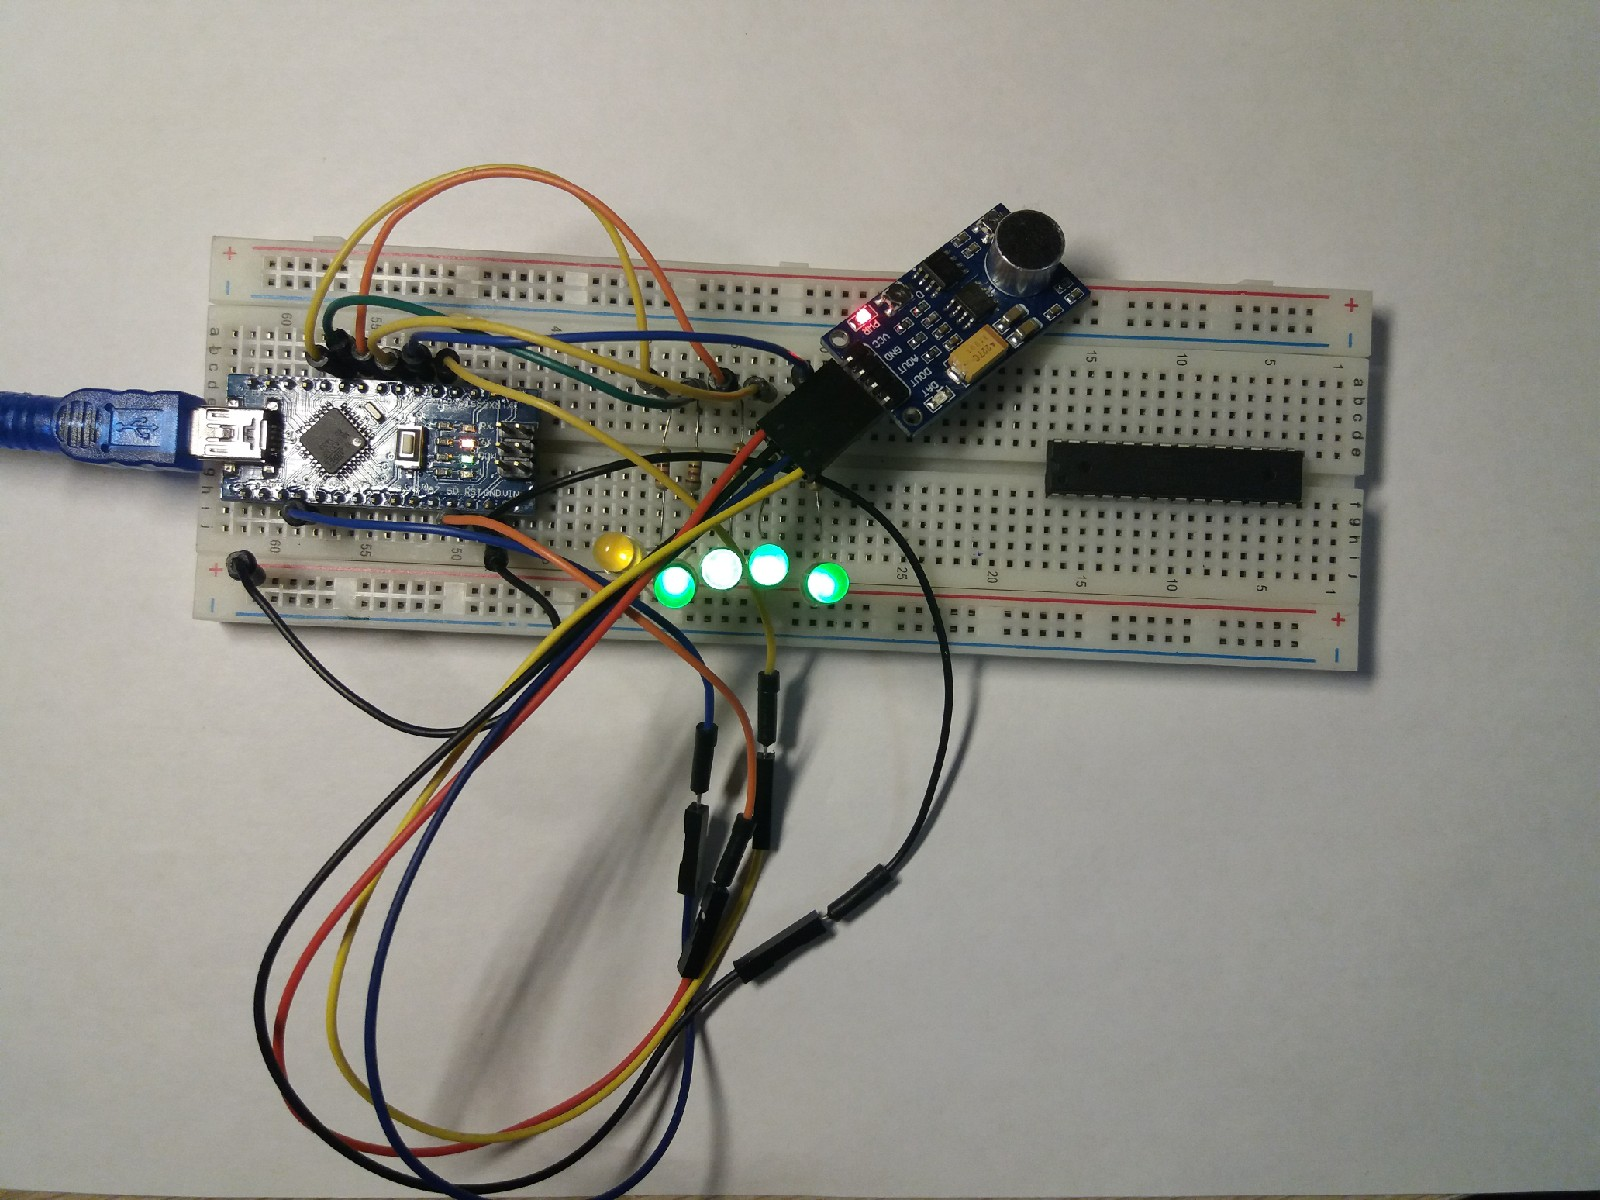
\includegraphics[width=1\linewidth]{mc}}
\end{figure}

\vfill

\hspace*{\fill}  Проект выполнили:\\
\hspace*{\fill}  Логовский Ян, 711 группа\\
\hspace*{\fill}  Чикунова Мария, 711 группа\\
\hspace*{\fill}  Кольцова Екатерина, 718 группа\\

\newpage

Идея проекта предельна проста:\\
\begin{enumerate}
\item{Измеряем интенсивность звука с помощью звукового модуля Ардуино}
\item{Микроконтроллер Ардуино Нано получает измеренное значение как аналоговый сигнал на один из своих входов, и, исходя из величины сигнала, подаёт напряжение на соответствующие выходы, из за чего загораются нужные светодиоды.}
\end{enumerate}
Код программы, загруженный в микроконтроллер:
\begin{lstlisting}
const int analogInPin  = A0;
int sensorAnalogValue  = 0;
const int digitalInPin = 2;
int sensorDigitalValue = 0;
const int level_1 = 7;
const int level_2 = 6;
const int level_3 = 5;
const int level_4 = 4;
const int level_5 = 3;
 
  
  
void setup() 
{
  Serial.begin(9600);
  Serial.println("Microphone Test" );
}

void loop() 
{
  int volume  = analogRead(analogInPin) - 500;
  
  
  if(volume < 20)
  {
    digitalWrite(level_1, HIGH);
    digitalWrite(level_2, LOW);
    digitalWrite(level_3, LOW);
    digitalWrite(level_4, LOW);
    digitalWrite(level_5, LOW);
  }
  if((volume >= 20) && (volume < 40))
  {
    digitalWrite(level_1, HIGH);
    digitalWrite(level_2, HIGH);
    digitalWrite(level_3, LOW);
    digitalWrite(level_4, LOW);
    digitalWrite(level_5, LOW);
  }
  if((volume >= 40) && (volume < 60))
  {
    digitalWrite(level_1, HIGH);
    digitalWrite(level_2, HIGH);
    digitalWrite(level_3, HIGH);
    digitalWrite(level_4, LOW);
    digitalWrite(level_5, LOW);
  }
  if((volume >= 60) && (volume < 80))
  {
    digitalWrite(level_1, HIGH);
    digitalWrite(level_2, HIGH);
    digitalWrite(level_3, HIGH);
    digitalWrite(level_4, HIGH);
    digitalWrite(level_5, LOW);
  }
  if((volume >= 80))
  {
    digitalWrite(level_1, HIGH);
    digitalWrite(level_2, HIGH);
    digitalWrite(level_3, HIGH);
    digitalWrite(level_4, HIGH);
    digitalWrite(level_5, HIGH);
  }
    
  Serial.print("Analog value= ");
  Serial.println(volume);
  
}
\end{lstlisting}




\end{document} % конец документа